\documentclass{article}
\usepackage{tikz}

\begin{document}
	
	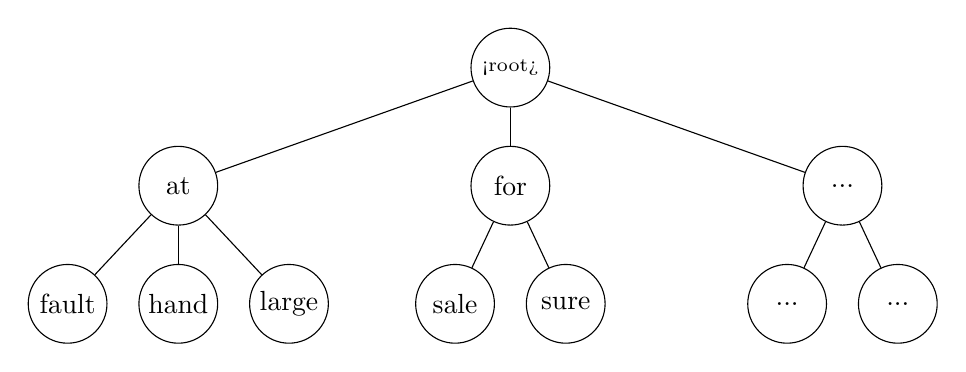
\begin{tikzpicture}[sibling distance=15em,
		every node/.style = {shape=circle, draw, align=center,
			text=black, fill=white, minimum size=1cm, inner sep=0pt},
		level 1/.style={sibling distance=12em},
		level 2/.style={sibling distance=4em}]
		
		\node {\scriptsize<root>}
		child { node {at}
			child { node {fault} }
			child { node {hand} }
			child { node {large} }}
		child { node {for}
			child { node {sale} }
			child { node {sure} }}
	child { node {...}
		child { node {...} }
		child { node {...} }};
	\end{tikzpicture}
	
	
	Let's define:
	
	\begin{itemize}
		\item \(S\) as the multiset for the input sentence.
		\item \(L\) as the set containing multisets, each representing a possible MWE, i.e., \(L = \{M_1, M_2, ..., M_n\}\) where each \(M_i\) is a multiset.
	\end{itemize}
	
	We want to find:
	
	\[
	L' = \{M \in L \ | \ M \subset S\}
	\]
	
	Here, \(M \subset S\) denotes that \(M\) is a strict subset of \(S\), meaning that all elements of \(M\) are contained in \(S\), and \(M\) is not equal to \(S\) (indicating it's a strict subset).
	
	\[
	\frac{\sum_{cw \in C} score(cw)}{\sum_{bw \in B} usageCount(bw)^2}
	\]
	
	
	
\end{document}
